\chapter{Design}
The overall goal for the design of the DSP and DSL was to allow for the greatest amount of flexibility, so the resulting DPS generated would require the minimum amount of space on the system.


\section{DSP}
The basis of the design comes from the QDSP designed by Anders Steengaard. This design was maintained in the VHDL as to support interoperability between the old and new design while additional features were added. The overall design of the DSP can be seen in \figref{fig:DSPDiagram}. The design was created to allow the DSP to be inserted in applications that use $\mu$TosNet or Unity-Link and only require minimal changes to the existing VHDL. The result of this design is that the DSP has two main memory areas, on to interface with the surrounding VHDL, called the IO memory, and one to either $\mu$TosNet or Unity-Link refereed to as the Shared memory.

\begin{figure}[h]
	\centering
		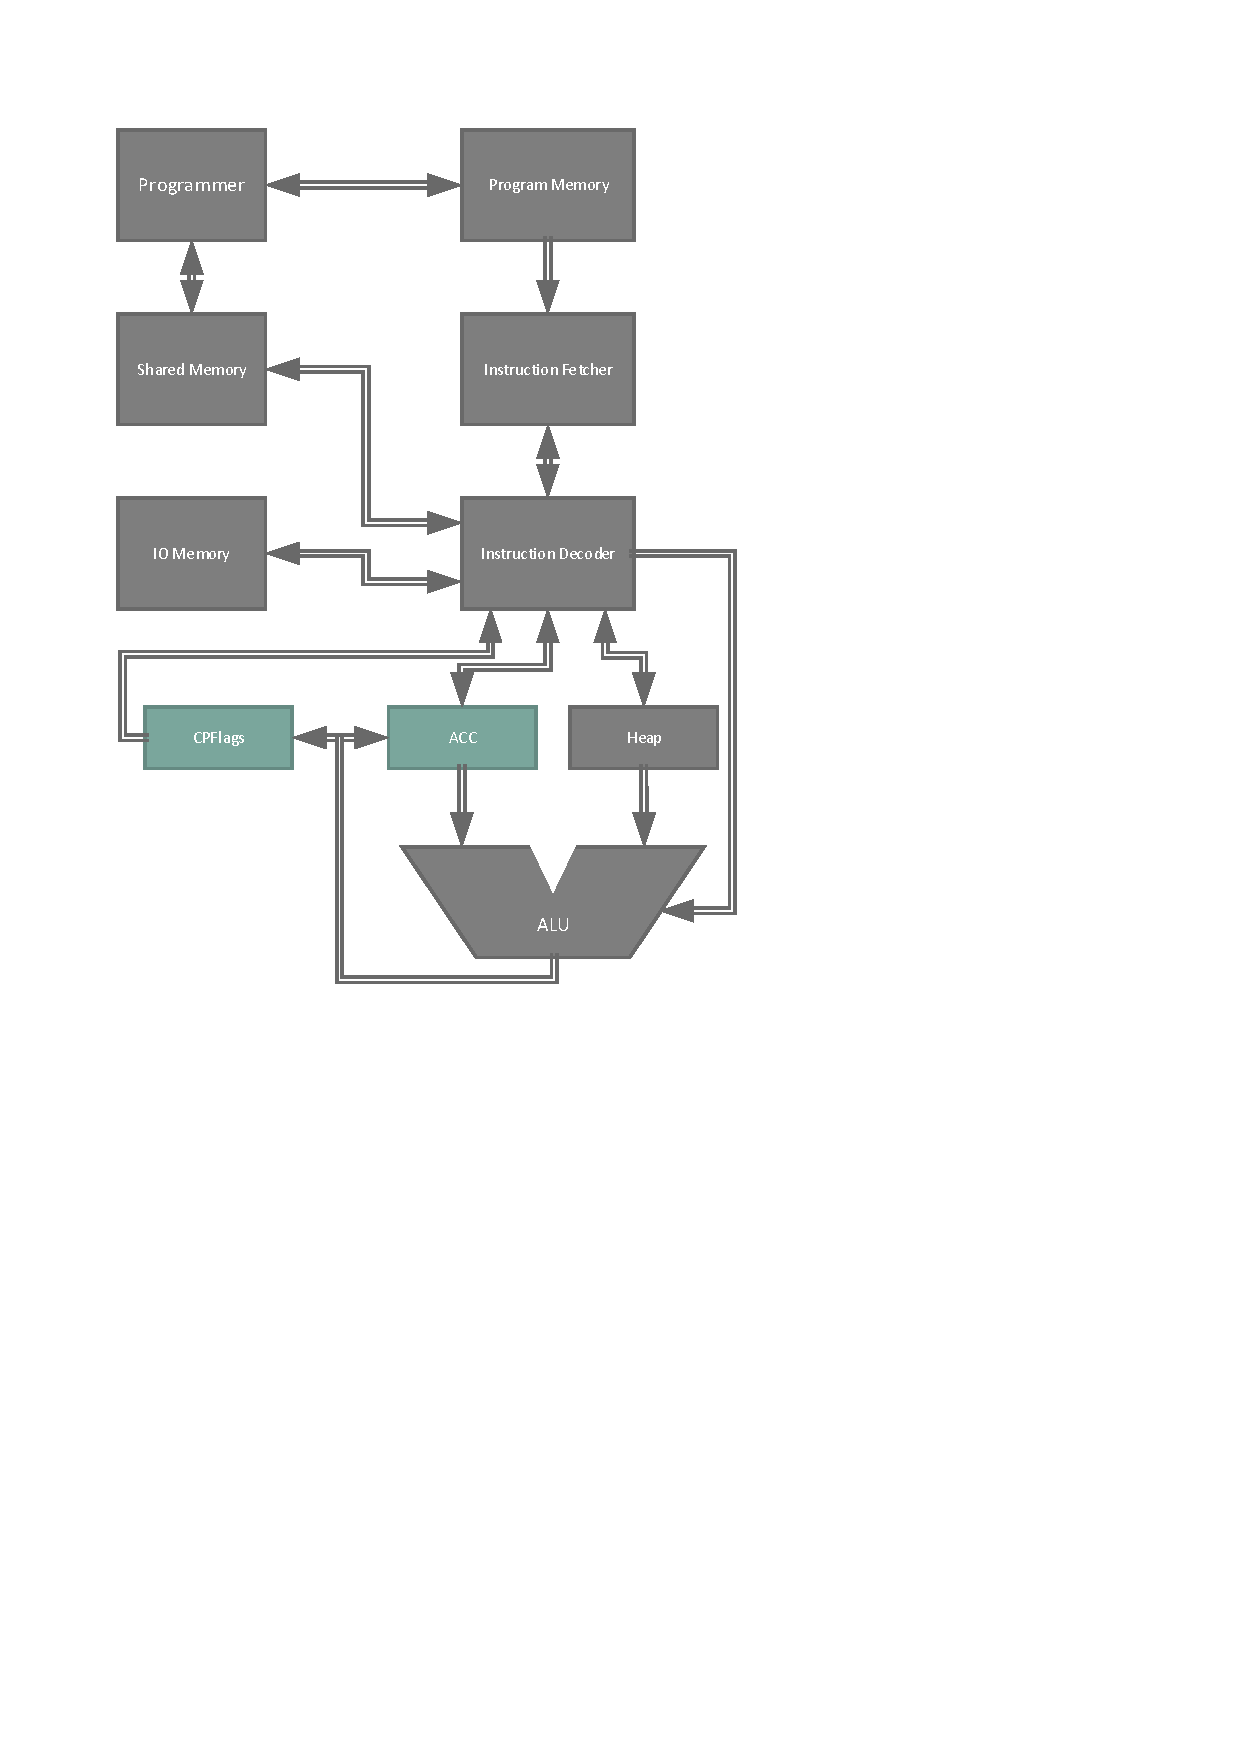
\includegraphics[width=0.40\textwidth]{../includes/pictures/DSPDiagram.pdf}
	\caption{Block diagram of QDSP}
	\label{fig:DSPDiagram}
\end{figure}

\subsection{Instruction-set}
The structure of the instruction-set from the original QDSP was designed to allow for arguments to be provided along with the instruction. This was done by having a fixed length instruction followed by argument, this structure was maintained in this new design.

The instruction-set was updated to allow for new features such as branching whereby evaluations on values could be done and subsequent jumps in the program code could be achieved, allowing for loops and conditional code execution.

Existing features of the old instruction-set such as the ability to divide or multiply by a fixed base2 number such as 256 using bit-shifting, was removed and an instruction that could do the same but also take an argument for the amount of bits to shift were put in their place, thus reducing the amount of instructions needed, when wanting to f.x. divide by two different numbers.

The full instruction-set can be found in \myref{appendix}{app:instruction-set}.

\section{Run-time programing}
Run-time programming functionality, designed to utilize the existing computer interface of the QDSP, was added to allow for the run-time programming the program memory, allowing for faster iterations on the code running on the DSP. To do this an additional component was added to the DSP that has access to the program memory and the shared memory, allowing it to circumvent the main instruction decoder. A file format was created to allow the compiler to create files that could be programmed to the device using a predetermined interface.
\subsection{Programming interface}
The programming interface was devised so it allowed for the programming of individual parts of the program and heap memory, as well as validation of the functionality of the device before programming in started. The interface uses four registers in on either µTosnet of Unity-Link, two to write data and two to receive. The complete command list can be seen in \tabref{tab:registers}.

\begin{table}[H]
\rowcolors{2}{table-gray}{}
	\centering
			\begin{tabular}{c||cc|c||cc|c}
		\textbf{Name} & \multicolumn{3}{c||}{\textbf{Transmit}} & \multicolumn{3}{c}{\textbf{Receive}}\\
		& \multicolumn{2}{c|}{\textbf{Control}} & \textbf{Data-Out} & \multicolumn{2}{c|}{\textbf{Status}} & \textbf{Data-In} \\ \hline
		%& \textbf{Command} & \textbf{Data} &  & \textbf{Command} & \textbf{Data} & \\ 
		start loader & 0x81 & N/A & N/A & 0x81 & N/A & N/A\\
		stop loader & 0x82 & N/A & N/A & N/A & N/A & N/A\\
		write program & 0x83 & Address & program data & 0x83 & Address & program data\\
		read program & 0x84 & Address & N/A & 0x84 & Address & program data \\
		write heap & 0x85 & Address & heap data & 0x85 & Address & heap data\\
		read heap & 0x86 & Address & N/A & 0x86 & Address & heap data \\
		validate device & 0x87 & Feature key & Validation key & 0x87 & Feature result & Validation result \\
	\end{tabular}
		\caption{List of commands used in the program loader.}
		\label{tab:registers}
\end{table}


The control and status registers uses the structure defined in \tabref{tab:controlregisters}, that allows extra data to be transmitted along side the command, and the Data-in and -out allows for the transmission of data to the DSP. The Start and Stop loaders commands are used to inform the DSP to go into the programming state. when the programming state is entered the is returned in the status register, but as the loader is stopped when a stop loader command is sent, not change on the status register is possible.

\begin{table}[H]
\rowcolors{2}{table-gray}{}
	\centering
			\begin{tabular}{c|c|l}
		\textbf{Start} & \textbf{Size[Byte]} & \textbf{Description} \\ \hline
		0 & 2 & command \\ 
		2 & 6 & data \\
	\end{tabular}
		\caption{Structure of control and Status registers.}
		\label{tab:controlregisters}
\end{table}

The read program and read heap commands uses the address provided in the control data area to return the address and data of a given memory area.
When writing a new program to the DSP first the validation must be performed, until that is done the loader is in a read only state. This is done by transmitting a validation command along with a feature key, this feature key is a on-hot encoding of all the instructions required by the code, and a validation key, which structure can be seen in \tabref{tab:validationkey}. These keys are validated on the DSP and the results are returned. If the validation was successful the read-only flag is removed allowing for the programming of the DSP.

\begin{table}[H]
\rowcolors{2}{table-gray}{}
	\centering
			\begin{tabular}{c|c|l}
		\textbf{Start} & \textbf{Size[Bit]} & \textbf{Description} \\ \hline
		0 & 10 & Heap size \\ 
		10 & 22 & Program size \\
	\end{tabular}
		\caption{Structure of the validation key and result.}
		\label{tab:validationkey}
\end{table}

The write program and heap commands requires the address that is to be written along side the data, when that is received the data is stored in the memory and the new address and data value is returned, allowing for validation of the written data.

\subsection{Programming file format}
\label{sec:design:binaryfile}
The programming file is designed to allow the programming software to get all parameters needed to successfully program the DSP. The data is stored in a binary format, consisting of a header followed  by the heap and program data. The overview of the file structure can be seen in \tabref{tab:binfile}. 

\begin{table}[H]
\rowcolors{2}{table-gray}{}
	\centering
			\begin{tabular}{c|c|c|l}
		\textbf{Start} & \textbf{Size[Byte]} & \textbf{Name} & \textbf{Description} \\ \hline
		0 & 1 & HS & Size of header\\ 
		1 & 1 & CA & Control Address \\ 
		2 & 1 & OA & Data-Out Address \\ 
		3 & 1 & IA & Data-In Address \\ 
		4 & 1 & SA & Status Address \\ 
		5 & 1 & PCL & Program Code Length \\ 
		6 & 2 & HC & Heap Count \\ 
		8 & 2 & PC & Program Count \\ 
		10 & 6 & FK & Feature Key \\ 
		16 & 8 & VK & Validation Key \\
		$HS$ & $5 \cdot HC$ & HD & Heap Data \\
		$HS + 5 \cdot HC$ & $PCL \cdot PC$ & PD & Program Data \\
		
	\end{tabular}
		\caption{Data structure of programming file}
		\label{tab:binfile}
\end{table}
\subsubsection{Headder}
The first data is used to determine the size of the header, which allows for changes to the header and still retain backwards compatibility. The next four elements describes what registers should be used for the communication. These are followed by the PCL element, which describes the size of each Program data element in bytes, this ensures that the program data occupies a minimum of space in the file. The heap and program count are used to calculate the start and end of the data areas, as they have no predefined length, but depends on the program created. Lastly the feature and validation keys that are used to ensure that the DSP supports the functions required of the program.

\subsubsection{Heap data}
The heap data is structured with an address and value, this means that only the heap elements that has initial values needs to be stored in the file and programmed. The structure can be seen in \tabref{tab:binheap}.
\begin{table}[H]
\rowcolors{2}{table-gray}{}
	\centering
			\begin{tabular}{c|c|l}
		\textbf{Start} & \textbf{Size[Byte]} & \textbf{Description} \\ \hline
		0 & 1 & Address \\ 
		1 & 4 & Value \\
	\end{tabular}
		\caption{Data structure of heap data element}
		\label{tab:binheap}
\end{table}
\subsubsection{Program data}
The program data stores the code for the entire program, stored sequentially this is done as there is no need to assign addresses to the programming code, as it will need to overwrite the entire code every time the DSP is programmed. The structure of a program data element can be seen in \tabref{tab:binprogram}.
\begin{table}[H]
	\centering
			\begin{tabular}{c|c|l}
		\textbf{Start} & \textbf{Size[Byte]} & \textbf{Description} \\ \hline
		0 & PCL & Value \\ 
	\end{tabular}
		\caption{Data structure of program data element}
		\label{tab:binprogram}
\end{table}

\section{Language}
There are generally two different ways of making DSLs. They can be either internal, where they are running inside of another language, and external, where a separate program is used and new files are generated. In the current project an external DSL was the most applicable. In order to facilitate the creation of the DSL eclipse with xtext was chosen as the development platform, as this allows for the creation of an eclipse plug-in. By doing this the DSL can later be written and complied in eclipse all the features of eclipse, such as syntax and error highlighting.

\subsection{General structure}
The overall structure of the language resembles C, thou utilizing a limited subset of the features, making it easier for anyone with experience with a C-like programming language to program to the QDSP. As the structure of the DSP is unique there are several differences that bares mentioning.

\subsubsection{Data formats}
The data formats that the language has are define, var, and constant.

\textbf{Constants} are used when defining a number that can not be changed later in the code.

\textbf{Defines} are used to give meaningful names to the memory addresses in the two main interfaces of the DSP i.e. the IO memory and Shared Memory

\textbf{Vars} are used when dealing with variables on the DSP, these occupy the heap, and the data can be changed anywhere in the program.

\subsubsection{Math operators}
The mathematical operators implemented thus far can be found in \tabref{tab:mathOperators}. These are selected as they are the basic mathematical operations needed to do most math. The order of operations chosen is purely based on the order of the operators, with no significance given to the type of operator used, this was chosen as it would require less time to implement, and allowed more focus on other parts of the design. In order to allow specific operations to be evaluated correct, support for parenthesis was included as this gave a greater freedom when writing the equations. 

\begin{savenotes}
	\begin{table}[H]
		\rowcolors{2}{table-gray}{}
		\centering
						\begin{tabular}{c|c}
				\textbf{Operator} & \textbf{Description}\\
				\hline
				+	& Add \\
				- & Subtract \\
				* & Multiply\footnote{The multiplier multiplies to values and stores the result in a 32 bit value make sure that the result dos not exceeds a 32 bit value.} \\
				/ & Divide\footnote{It is only possible to divide by a number that is a power of 2. It is therefore not possible to divide by variables and constants.} \\
				<< & Left bit shift \\
				>> & Right bit shift
			\end{tabular}
			\caption{Math operators}
		\label{tab:mathOperators}
	\end{table}
\end{savenotes}

There are some caveats with some of the operators, namely the multiplication and division. The multiplication only outputs its result into the same signed 32bit values as all data elements, this requires the user to ensure that the result does not exceed this when calculating, as data will be lost. The division used in the design is based on bit-shifting as this can be done on one clock cycle but the downside to this is it only supports division with numbers that are a power of two.

\subsubsection{Assignment operators}
The assignment operators that are implemented is a natural extension of the supported mathematical operators, as they are dependent on the mathematical operators. A list of the assignment operators can be found in \tabref{tab:assignmentOperators}.
\begin{table}[H]
	\rowcolors{2}{table-gray}{}
	\centering
			\begin{tabular}{c|c}
		\textbf{Operator} & \textbf{Description}\\
		\hline
		=  & Sets the data to the argument\\
		+= & Adds the argument\\
		-= & Subtracts the argument\\
		*= & Multiplys with the argument\\
		++ & Adds 1 \\
		{-}- & Subtracts 1 
	\end{tabular}
		\caption{Assignment operators}
		\label{tab:assignmentOperators}
\end{table}

\subsection{Custom functions}
In addition to the normal c-like options of language several custom functions have been added to enable some of the more specific features of the DSP, they can be seen in \tabref{tab:configurations}. 
\begin{table}[H]
	\rowcolors{2}{table-gray}{}
	\centering
				\begin{tabular}{c|c|l}
		\textbf{Name} & Format & \textbf{Description} \\
		Min & \mono{Min(x,y)} & Finds and returns the lowest value of x and y \\
		Max & \mono{Max(x,y)} & Finds and returns the largest value of x and y \\
		Sleep & \mono{Sleep(x)} & Inserts x amount of NOPs in the program code \\
		trunctate16 & \mono{trunctate16(x)} & Truncates the number to a 16bit value \\
		RunBootLoader & \mono{RunBootLoader()} & Makes the code test if run-time programming is reqsted \\
		\end{tabular}
		\caption{Custom functions}
		\label{tab:customfunctions}
\end{table}
This is done as most of these map directly to instructions in the instruction set and does not have a natural way to be included with normal mathematical operations. The only function that does not map directly to a instruction is the sleep function, which adds a number of NOP operations to the code.

\subsection{Configuration}

In addition to the functional code the language also has parameters that can be used to adjust how the compiler processes the code. These are included in the language as opposed to having as parameters in the project, as this solution did not require an in-depth analysis into how eclipse stores project settings and allows an entire project to be contained within a single file. The entire list of parameters can be seen in \tabref{tab:configurations}

\begin{savenotes}
	\begin{table}[H]
		\rowcolors{2}{table-gray}{}
		\centering
			\begin{tabular}{c|c|c|p{6.6cm}}
	\textbf{Name} & \textbf{Type} & \textbf{Default} & \textbf{Description}\\
	\hline
	ProjectTitle & String & NewQdsp & Title of the project\\
	AutoCommentQDSPCode & Boolean & true & Comments the micro instructions\\
	EnableOptimization & Boolean & true & Assigns the programing transmit address on SH memory for run time programming\\
	RuntimeProgrammable & Boolean & false & Enables the capability of run time program the QDSP\\
	HeapSize\footnotemark\addtocounter{footnote}{-1}\addtocounter{Hfootnote}{-1} & Integer & 32 & The amount of Heap registers.\\
	ProgramMemorySize\footnotemark\addtocounter{footnote}{-1}\addtocounter{Hfootnote}{-1} & Integer & 128 & The amount of program memory available.\\
	ProgramingControlAddress\footnotemark\addtocounter{footnote}{-1}\addtocounter{Hfootnote}{-1} & Integer & 7 & Assigns the programing control address on SH memory for run time programming\\
	ProgramingStatusAddress\footnotemark\addtocounter{footnote}{-1}\addtocounter{Hfootnote}{-1} & Integer & 0 & Assigns the programing status address on SH memory for run time programming\\
	ProgramingDataInAddress\footnotemark\addtocounter{footnote}{-1}\addtocounter{Hfootnote}{-1} & Integer & 1 & Assigns the programing revise address on SH memory for run time programming\\
	ProgramingDataOutAddress\footnotemark\addtocounter{footnote}{-1}\addtocounter{Hfootnote}{-1} & Integer & 6 & \\
	SHInterfaceType\footnotemark & String & Unity-Link & Changes the SH interface to match Unity-Link or uTosNet \\
\end{tabular}
\footnotetext{Only used if RuntimeProgrammable it true}
			\caption{Configuration paramaters}
		\label{tab:configurations}
	\end{table}
\end{savenotes}

